

% Gradient Info
  
\tikzset {_e292ujfi3/.code = {\pgfsetadditionalshadetransform{ \pgftransformshift{\pgfpoint{513 bp } { -174 bp }  }  \pgftransformscale{3 }  }}}
\pgfdeclareradialshading{_n7edsi42z}{\pgfpoint{-176bp}{64bp}}{rgb(0bp)=(1,1,1);
rgb(0bp)=(1,1,1);
rgb(12.767857142857142bp)=(0.91,0.25,0.25);
rgb(400bp)=(0.91,0.25,0.25)}
\tikzset{every picture/.style={line width=0.75pt}} %set default line width to 0.75pt        

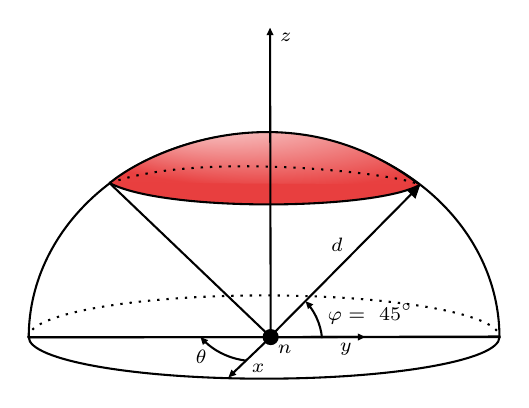
\begin{tikzpicture}[x=0.75pt,y=0.75pt,yscale=-1,xscale=1]
%uncomment if require: \path (0,300); %set diagram left start at 0, and has height of 300

%Shape: Chord [id:dp241657055871786] 
\draw   (193.93,190.4) .. controls (194.07,136.1) and (244.83,92.15) .. (307.4,92.19) .. controls (369.93,92.23) and (420.61,136.21) .. (420.74,190.46) -- cycle ;
%Curve Lines [id:da7774614939439684] 
\draw [shading=_n7edsi42z,_e292ujfi3]   (232.9,116.25) .. controls (253.33,99.17) and (321.67,70.17) .. (382.5,117.25) ;
%Shape: Boxed Bezier Curve [id:dp976459988898636] 
\draw [fill={rgb, 255:red, 232; green, 63; blue, 63 }  ,fill opacity=1 ]   (232.5,116) .. controls (246.19,123.48) and (280.95,126.81) .. (314,126.48) .. controls (325.54,126.36) and (336.87,125.79) .. (347.02,124.8) .. controls (363.03,123.24) and (376.13,120.61) .. (382.5,117) ;
%Shape: Circle [id:dp060964936174491724] 
\draw  [fill={rgb, 255:red, 0; green, 0; blue, 0 }  ,fill opacity=1 ] (307.13,190.4) .. controls (307.13,188.54) and (308.64,187.03) .. (310.51,187.03) .. controls (312.37,187.03) and (313.88,188.54) .. (313.88,190.4) .. controls (313.88,192.27) and (312.37,193.78) .. (310.51,193.78) .. controls (308.64,193.78) and (307.13,192.27) .. (307.13,190.4) -- cycle ;
%Straight Lines [id:da1793972926995161] 
\draw    (232.9,116.25) -- (247.22,129.93) -- (310.51,190.4) ;
%Straight Lines [id:da6269963502636927] 
\draw    (380.39,119.38) -- (308.38,192.13) ;
\draw [shift={(382.5,117.25)}, rotate = 134.71] [fill={rgb, 255:red, 0; green, 0; blue, 0 }  ][line width=0.08]  [draw opacity=0] (6.25,-3) -- (0,0) -- (6.25,3) -- cycle    ;
%Straight Lines [id:da5790726192958345] 
\draw    (310.51,190.4) -- (353.08,190.39) ;
\draw [shift={(356.08,190.39)}, rotate = 179.98] [fill={rgb, 255:red, 0; green, 0; blue, 0 }  ][line width=0.08]  [draw opacity=0] (3.57,-1.72) -- (0,0) -- (3.57,1.72) -- cycle    ;
%Shape: Arc [id:dp6972628103446205] 
\draw  [draw opacity=0] (327.33,173.18) .. controls (329.4,175.4) and (331.16,177.98) .. (332.51,180.87) .. controls (334.05,184.13) and (334.94,187.53) .. (335.24,190.93) -- (305.36,193.62) -- cycle ; \draw    (329.27,175.5) .. controls (330.51,177.14) and (331.6,178.93) .. (332.51,180.87) .. controls (334.05,184.13) and (334.94,187.53) .. (335.24,190.93) ;  \draw [shift={(327.33,173.18)}, rotate = 47.09] [fill={rgb, 255:red, 0; green, 0; blue, 0 }  ][line width=0.08]  [draw opacity=0] (3.57,-1.72) -- (0,0) -- (3.57,1.72) -- cycle    ;
%Straight Lines [id:da5528525747103438] 
\draw    (310.21,44.4) -- (310.51,190.4) ;
\draw [shift={(310.2,41.4)}, rotate = 89.88] [fill={rgb, 255:red, 0; green, 0; blue, 0 }  ][line width=0.08]  [draw opacity=0] (3.57,-1.72) -- (0,0) -- (3.57,1.72) -- cycle    ;
%Straight Lines [id:da8340088843622058] 
\draw    (292.37,207.73) -- (310.51,190.4) ;
\draw [shift={(290.2,209.8)}, rotate = 316.31] [fill={rgb, 255:red, 0; green, 0; blue, 0 }  ][line width=0.08]  [draw opacity=0] (3.57,-1.72) -- (0,0) -- (3.57,1.72) -- cycle    ;
%Curve Lines [id:da6149455400699015] 
\draw  [dash pattern={on 0.84pt off 2.51pt}]  (232.9,116.25) .. controls (277.35,100.09) and (376.33,112.17) .. (382.5,117.25) ;
%Shape: Pie [id:dp4766908428725254] 
\draw   (420.72,190.14) .. controls (420.73,190.25) and (420.74,190.36) .. (420.74,190.46) .. controls (420.74,201.51) and (369.96,210.46) .. (307.33,210.46) .. controls (244.78,210.46) and (194.05,201.53) .. (193.93,190.5) -- (307.33,190.46) -- cycle ;
%Shape: Arc [id:dp28428573759108733] 
\draw  [draw opacity=0][dash pattern={on 0.84pt off 2.51pt}] (193.97,190.87) .. controls (193.94,190.69) and (193.93,190.51) .. (193.93,190.34) .. controls (193.93,179.29) and (244.7,170.34) .. (307.33,170.34) .. controls (366.46,170.34) and (415.02,178.32) .. (420.27,188.5) -- (307.33,190.34) -- cycle ; \draw  [dash pattern={on 0.84pt off 2.51pt}] (193.97,190.87) .. controls (193.94,190.69) and (193.93,190.51) .. (193.93,190.34) .. controls (193.93,179.29) and (244.7,170.34) .. (307.33,170.34) .. controls (366.46,170.34) and (415.02,178.32) .. (420.27,188.5) ;  
%Shape: Arc [id:dp41874576724679013] 
\draw  [draw opacity=0] (298.58,201.75) .. controls (292.94,201.07) and (287.32,199.03) .. (282.43,195.59) .. controls (280.23,194.04) and (278.32,192.3) .. (276.71,190.44) -- (299.99,176.96) -- cycle ; \draw    (298.58,201.75) .. controls (292.94,201.07) and (287.32,199.03) .. (282.43,195.59) .. controls (281.1,194.65) and (279.88,193.65) .. (278.76,192.58) ; \draw [shift={(276.71,190.44)}, rotate = 47.4] [fill={rgb, 255:red, 0; green, 0; blue, 0 }  ][line width=0.08]  [draw opacity=0] (3.57,-1.72) -- (0,0) -- (3.57,1.72) -- cycle    ; 

% Text Node
\draw (338.16,141.1) node [anchor=north west][inner sep=0.75pt]  [font=\scriptsize] [align=left] {$\displaystyle d$};
% Text Node
\draw (312.51,193) node [anchor=north west][inner sep=0.75pt]  [font=\scriptsize] [align=left] {$\displaystyle n$};
% Text Node
\draw (300,202) node [anchor=north west][inner sep=0.75pt]  [font=\scriptsize] [align=left] {$\displaystyle x$};
% Text Node
\draw (342.37,192) node [anchor=north west][inner sep=0.75pt]  [font=\scriptsize] [align=left] {$\displaystyle y$};
% Text Node
\draw (313.59,42.6) node [anchor=north west][inner sep=0.75pt]  [font=\scriptsize] [align=left] {$\displaystyle z$};
% Text Node
\draw (336.4,172.8) node [anchor=north west][inner sep=0.75pt]  [font=\scriptsize] [align=left] {$\displaystyle \varphi =\ 45^{\circ }$};
% Text Node
\draw (272.8,195.4) node [anchor=north west][inner sep=0.75pt]  [font=\scriptsize] [align=left] {$\displaystyle \theta $};


\end{tikzpicture}
